\section{Quantitative Violation Semantics}

\subsection{Motivation and Scope}

\paragraph{Beyond Binary Verdicts.}
The fundamental limitation of the forward-looking tight satisfaction semantics, as defined in the previous section, lies in its binary and prefix-closed nature.
In that framework, the monitoring process halts definitively at the first tight violation.
While computationally efficient for stopping enforcement mechanisms (e.g., access control), this ``first-fail'' approach is insufficient for post-hoc auditing or dispute resolution.
It masks the full history of non-compliance, failing to capture cumulative violations or distinct failures by multiple agents over time—a critical requirement for comprehensive legal accountability.
To address this, we must transition from a boolean verdict to a \emph{quantitative semantics}, moving from the question ``Did a violation occur?'' to ``How many violations occurred, and of what magnitude?''


\paragraph{The Challenge of Temporal Scope.}
A prerequisite for counting violations is defining the temporal window over which the contract is evaluated.
Unlike traditional model checking where traces are often infinite, contract monitoring operates on finite, evolving prefixes.
We identify two primary strategies for defining this scope:

\begin{enumerate}
    \item \textbf{Static Pre-computation:} One might attempt to calculate a fixed duration $T$ for a contract $C$.
    However, contracts containing unbounded repetitions ($\repit{C}$) or input-dependent regular expressions (guards/triggers) do not have a statically determinable length.
   
    \item \textbf{Dynamic On-the-Fly Detection:} The alternative is to determine the contract's status dynamically at every step.
    Here, the monitor continuously computes a \emph{residual contract}—a formula representing what remains to be fulfilled given the history of events.
   
\end{enumerate}

In this work, we adopt the \textbf{Dynamic On-the-Fly} approach.
This requires a structural tracking mechanism, which we formalize as the \emph{Contract Progress Monitor} (CPM).
The CPM acts as a derivative function: given a contract $C$ and an incoming event, it computes the contract $C'$ that must be enforced in the next time step.
By isolating the \emph{state} of the contract (via the CPM) from the \emph{evaluation} of compliance (via a scoring function), we enable a modular framework that can track active duties, handle contrary-to-duty (CTD) transitions, and attribute blame precisely over time.


\subsection{Contract Progress Monitor}

The core of our quantitative framework is the \emph{progression function}, $\Prog$.
Conceptually similar to the Brzozowski derivative~\cite{brzozowski1964derivatives} for regular expressions, $\Prog$ consumes the current event and the current contract to produce the \emph{residual contract} for the subsequent step.

\begin{definition}[Contract Progression Function]
Let $\Gamma = 2^\Sigma$ be the event alphabet.
We extend the set of contracts $\mathcal{C}$ with a distinguished symbol $\emptc$, representing a \emph{discharged contract} (one that implies no further obligations).

The progression function $\Prog: \Gamma^* \times \cDL \to \cDL \cup \{\emptc\}$ is defined recursively.
For the empty trace $\epsilon$, $\Prog(\epsilon, C) := C$.
For a single event step $\trace{A}$ with $A \in \Gamma$, the function is defined on the structure of $C$ as follows.

\paragraph{Literals (State Update).}
For any literal $\ell$ (obligation, permission, or prohibition):
\[
\Prog(\trace{A}, \ell) := \emptc
\]
\emph{Rationale:} Structurally, a literal applies to a single time step.
Once that step $A$ occurs, the literal is consumed.
Whether $A$ satisfied or violated $\ell$ is immaterial to the \emph{progression} (the duty is passed); the violation is recorded separately by the quantitative scoring function defined later.


\paragraph{Conjunction (Parallel Progress).}
\[
\Prog(\trace{A}, C_1 \wedge C_2) := \Prog(\trace{A}, C_1) \wedge \Prog(\trace{A}, C_2)
\]
We assume the algebraic identity where $\emptc$ is the neutral element for conjunction: $\emptc \wedge C' \equiv C'$.


\paragraph{Sequence (Sequential Handover).}
For a sequence $C_1 ; C_2$, progression determines if the current step concludes $C_1$:
\[
\Prog(\trace{A}, C_1 ; C_2) := 
\begin{cases}
  \Prog(\trace{A}, C_1) ; C_2 & \text{if } \Prog(\trace{A}, C_1) \neq \emptc, \\
  \Prog(\trace{A}, C_2) & \text{if } \Prog(\trace{A}, C_1) = \emptc.
\end{cases}
\]
If $C_1$ is discharged by step $A$ (i.e., its residual is $\emptc$), the monitor immediately activates the first step of the continuation $C_2$.


\paragraph{Reparation (Contrary-to-Duty Branching).}
The reparation construct is unique because its structural evolution depends on the satisfaction of the primary obligation.
This is the only case where $\Prog$ relies on the tight satisfaction relation ($\satt, \violt, \presat$) to determine the path:
\[
\Prog(\trace{A}, C_1 \repair C_2) := 
\begin{cases}
  \Prog(\trace{A}, C_1) \repair C_2 & \text{if } \trace{A} \presat C_1 \text{ (Pending)}, \\
  \Prog(\trace{A}, C_2) & \text{if } \trace{A} \violt C_1 \text{ (Violation $\to$ Repair)}, \\
  \emptc & \text{if } \trace{A} \satt C_1 \text{ (Satisfaction $\to$ Discharge)}.
\end{cases}
\]
If a violation occurs ($\trace{A} \violt C_1$), the primary contract is discarded, and the secondary contract $C_2$ is activated immediately for the \emph{next} step.


\paragraph{Repetition.}
Repetition unrolls the contract one step at a time:
\[
\Prog(\trace{A}, \repit{C}) := \Prog(\trace{A}, C) ; \repit{C}
\]


\paragraph{Guarded and Triggered Contracts.}
These constructs rely on regular expression matching.
\[
\Prog(\trace{A}, \guard[re]{C}) :=
\begin{cases}
  \emptc & \text{if } \trace{A} \satt \guard[re]{C} \text{ (Guard satisfies, release)}, \\
  \guard[\Prog_{re}(\trace{A}, re)]{\Prog(\trace{A}, C)} & \text{otherwise (Guard persists)}.
\end{cases}
\]
\[
\Prog(\trace{A}, \trig[re]{C}) :=
\begin{cases}
  \emptc & \text{if } \trace{A} \violt re \text{ (Trigger failed permanently)}, \\
  C & \text{if } \trace{A} \satt re \text{ (Trigger fires)}, \\
  \trig[\Prog_{re}(\trace{A}, re)]{C} & \text{if } \trace{A} \presat re \text{ (Trigger pending)}.
\end{cases}
\]


\paragraph{Regular Expression Derivatives ($\Prog_{re}$).}
The helper function $\Prog_{re}$ computes the standard derivative~\cite{brzozowski1964derivatives} of the regular expression.
For atomic sets $A'$ and step $A$, $\Prog_{re}(\trace{A}, A') = \epsilon$ if matches, else failure.
For operations like union ($\mid$) and Kleene plus ($^+$), the derivatives follow standard automata-theoretic constructions.


\end{definition}

\begin{lemma}[Termination]
For any finite prefix $\pi$, $\Prog(\pi, C)$ terminates in at most $|\pi|$ recursive steps.

\end{lemma}
To illustrate the CPM, we examine how the residual contract evolves under different traces. We begin with the fundamental building block of normative enforcement: the reparation.

\begin{example}[Progression of Reparation]
\label{ex:prog-repit}
Consider the basic rental reparation clause:
\[ C_3 := \obl[1]{\PAY}\ \repair\ \obl[1]{\PAYF}. \]

\noindent\textbf{Scenario 1: Compliance.}
In the first trace $\pi$, the tenant pays rent in Month 1 ($\PAY \in A_1$). Since $\trace{A_1} \satt \obl[1]{\PAY}$, the condition for discharge is met. The reparation structure collapses to $\emptc$, meaning no further obligations exist for Month 2.

    \boxalignfigure{\resizebox{0.7\textwidth}{!}{%
    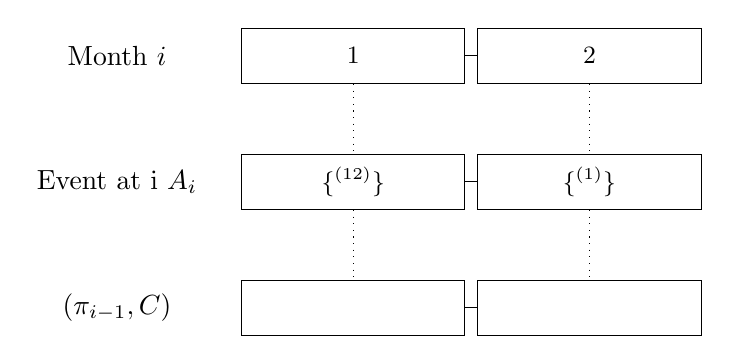
\begin{tikzpicture}[y=1.6cm,x=3.0cm]
    
      \tikzset{
        cell/.style={
          draw, rectangle, text width=26mm,
          minimum height=7mm, align=center, font=\small
        }
      }
    
      % Labels
      \node at (0,0)   {Month $i$};
      \node at (0,-1)  {Event at i $A_i$};
      \node at (0,-2)  {$\Prog(\pi_{i-1},C)$};
      % Row 1: time
      \node[cell] at (1,0) (t1) {$1$};
      \node[cell] at (2,0) (t2) {$2$};
      % Row 2: events
      \node[cell] at (1,-1) (e1) {$\{\PAY^{(12)}\}$};
      \node[cell] at (2,-1) (e2) {$\{\OCC^{(1)}\}$};
      % Row 3: residuals
      \node[cell] at (1,-2) (r1) {\emptc};
      \node[cell] at (2,-2) (r2) {\emptc};
      % Arrows
      \draw (t1)--(t2);
      \draw (e1)--(e2);
      \draw (r1)--(r2);
      % Vertical alignment
      \draw[dotted](t1.south)--(e1.north);
      \draw[dotted](e1.south)--(r1.north);
    
      \draw[dotted](t2.south)--(e2.north);
      \draw[dotted](e2.south)--(r2.north);
    \end{tikzpicture}
    }}
    {Progression on $ \obl[1]{\PAY}\ \repair\ \obl[1]{\PAYF}$ with a trace for which a no reparation is not required}
    {example:prog-repair1}
    {\vspace{8pt}}{\vspace{-12pt}}

\medskip
\noindent\textbf{Scenario 2: Violation and Repair.}
In trace $\pi'$, the tenant fails to pay in Month 1 ($\PAY \notin A'_1$). Here, $\trace{A'_1} \violt \obl[1]{\PAY}$. Consequently, the CPM activates the repair branch. The residual for Month 2 becomes $\obl[1]{\PAYF}$, obliging the tenant to pay the fine.

  \boxalignfigure{\resizebox{0.7\textwidth}{!}{%
  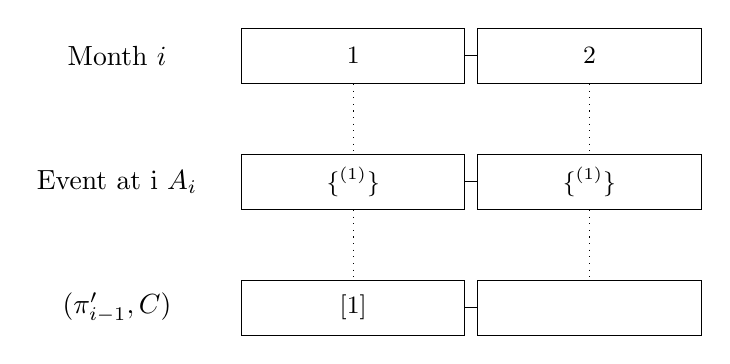
\begin{tikzpicture}[y=1.6cm,x=3.0cm]
  
    \tikzset{
      cell/.style={
        draw, rectangle, text width=26mm,
        minimum height=7mm, align=center, font=\small
      }
    }
  
    % Labels
    \node at (0,0)   {Month $i$};
    \node at (0,-1)  {Event at i $A_i$};
    \node at (0,-2)  {$\Prog(\pi'_{i-1},C)$};
    % Row 1: time
    \node[cell] at (1,0) (t1) {$1$};
    \node[cell] at (2,0) (t2) {$2$};
    % Row 2: events
    \node[cell] at (1,-1) (e1) {$\{\OCC^{(1)}\}$};
    \node[cell] at (2,-1) (e2) {$\{\OCC^{(1)}\}$};
    % Row 3: residuals
    \node[cell] at (1,-2) (r1) {$\obl[1]{\PAYF}$};
    \node[cell] at (2,-2) (r2) {\emptc};
    % Arrows
    \draw (t1)--(t2);
    \draw (e1)--(e2);
    \draw (r1)--(r2);
  
    % Vertical alignment
    \draw[dotted](t1.south)--(e1.north);
    \draw[dotted](e1.south)--(r1.north);
  
    \draw[dotted](t2.south)--(e2.north);
    \draw[dotted](e2.south)--(r2.north);
  
  \end{tikzpicture}
  }}
  {Progression on $ \obl[1]{\PAY}\ \repair\ \obl[1]{\PAYF}$ with a trace for which a no reparation is not required}
  {example:prog-repair2}
  {\vspace{8pt}}{\vspace{-12pt}}
\end{example}

Having established how single-step reparations evolve, we now extend the analysis to ongoing contracts. The following example demonstrates how the CPM handles infinite streams where duties recur every month, showing how violations in one period persist into the next.

\begin{example}[Progression of Infinite Repetition]
Consider the recurring contract $\repit{C_3}$, where the tenant must pay rent (or a fine) every month.
\[ \repit{C_3} = \repit{ \obl[1]{\PAY}\ \repair\ \obl[1]{\PAYF}}. \]

\noindent\textbf{Trace Analysis.}
We observe a trace where the tenant pays in Month 1 but fails to pay in Month 2 (occupying instead).
\begin{itemize}
    \item \textbf{Step 1 ($A_1$):} The tenant pays. The instance of $C_3$ for Month 1 is discharged. Due to the repetition operator, the residual is $\emptc ; \repit{C_3} \equiv \repit{C_3}$. The contract effectively ``resets'' for the next month.
    \item \textbf{Step 2 ($A_2$):} The tenant occupies but does not pay. The instance of $C_3$ for Month 2 is violated. Unlike Step 1, the residual does not reset cleanly. Instead, the violated obligation transforms into its reparation $\obl[1]{\PAYF}$, which must be fulfilled in the \emph{next} step (Month 3), alongside the continuing repetition $\repit{C_3}$.
\end{itemize}
This results in an accumulation of duties: the fine from Month 2 and the new rent for Month 3.

  \boxalignfigure{\resizebox{0.7\textwidth}{!}{%
  \begin{tikzpicture}[y=1.6cm,x=3.0cm]
  
    \tikzset{
      cell/.style={
        draw, rectangle, text width=26mm,
        minimum height=7mm, align=center, font=\small
      }
    }
  
    % Labels
    \node at (0,0)   {Month $i$};
    \node at (0,-1)  {Event at i $A_i$};
    \node at (0,-2)  {$\Prog(\pi_{i-1},C)$};
    % Row 1: time
    \node[cell] at (1,0) (t1) {$1$};
    \node[cell] at (2,0) (t2) {$2$};
    % Row 2: events
    \node[cell] at (1,-1) (e1) {$\{\PAY^{(12)}\}$};
    \node[cell] at (2,-1) (e2) {$\{\OCC^{(1)}\}$};
    % Row 3: residuals
    \node[cell] at (1,-2) (r1) {$\repit{C_3}$};
    \node[cell] at (2,-2) (r2) {$\obl[1]{\PAYF} ; \repit{C_3}$};
    % Arrows
    \draw (t1)--(t2);
    \draw (e1)--(e2);
    \draw (r1)--(r2);
  
    % Vertical alignment
    \draw[dotted](t1.south)--(e1.north);
    \draw[dotted](e1.south)--(r1.north);
  
    \draw[dotted](t2.south)--(e2.north);
    \draw[dotted](e2.south)--(r2.north);
  
  \end{tikzpicture}
  }}
  {Progression on $\repit{C_3}$ where the obligation is met in the first month but violated in the second.}
  {example:prog-repitc1}
  {\vspace{8pt}}{\vspace{-12pt}}
\end{example}

While repetitions capture simple recurring duties, more complex contracts are often bounded by conditions. Finally, we examine how the CPM handles \emph{guarded contracts}, where the outer structure (the guard) and the inner structure (the obligations) evolve independently until a termination event occurs.

\begin{example}[Progression of Guarded Contracts]
We examine a guarded contract that persists until a termination notice ($\notifterm$) is issued.
\[ \guard[\Gamma^+ \cdot \notifterm^{(1)}]{\repit{C_3}} \]

\noindent\textbf{Trace 1: Successful Termination.}
The tenant pays in Month 1 ($A_1$) and issues a termination notice in Month 2 ($A_2$).
\begin{itemize}
    \item At $i=1$, the event $A_1$ satisfies the inner contract $C_3$ (rent paid), but does not satisfy the guard (no notice). The residual is the guarded repetition.
    \item At $i=2$, the event $A_2$ contains $\notifterm$. This satisfies the guard expression. The CPM immediately reduces the entire contract to $\emptc$, signifying the contract has ended.
\end{itemize}

  \boxalignfigure{\resizebox{0.85\textwidth}{!}{%
  \begin{tikzpicture}[y=1.8cm,x=3.8cm]
  
    \tikzset{
      cell/.style={
        draw, rectangle, text width=34mm,
        minimum height=8mm, align=center, font=\small
      }
    }
    % Local definition for the residual regex to fit in the box
    \def\resid{\notifterm \mid \Gamma^+ \cdot \notifterm}
  
    % Labels
    \node at (0,0)   {Month $i$};
    \node at (0,-1)  {Event at i $A_i$};
    \node at (0,-2)  {$\Prog(\pi_{i-1},C)$};
    % Row 1: time
    \node[cell] at (1,0) (t1) {$1$};
    \node[cell] at (2,0) (t2) {$2$};
    % Row 2: events
    \node[cell] at (1,-1) (e1) {$\{\PAY^{(1)}, \PAY^{(2)}\}$};
    \node[cell] at (2,-1) (e2) {$\{\OCC^{(1)}, \notifterm^{(1)}\}$};
    % Row 3: residuals
    % Step 1: Contract satisfied (payment made), Guard not satisfied yet (needs >0 length or specific event).
    % Residual guard becomes (Notif | Gamma+ . Notif)
    \node[cell] at (1,-2) (r1) {$\guard[\resid]{\repit{C_3}}$};
    % Step 2: Guard satisfied by NotifTerm in A2. Contract discharges to epsilon.
    \node[cell] at (2,-2) (r2) {\emptc};
    % Arrows
    \draw (t1)--(t2);
    \draw (e1)--(e2);
    \draw (r1)--(r2);
  
    % Vertical alignment
    \draw[dotted](t1.south)--(e1.north);
    \draw[dotted](e1.south)--(r1.north);
  
    \draw[dotted](t2.south)--(e2.north);
    \draw[dotted](e2.south)--(r2.north);
  
  \end{tikzpicture}
  }}
  {Progression on guarded contract where the termination notice at step 2 discharges the contract.}
  {example:prog-guard1}
  {\vspace{8pt}}{\vspace{-12pt}}

\medskip
\noindent\textbf{Trace 2: Pending Guard with Internal Violation.}
In this scenario, the tenant pays in Month 1 but fails to pay (and gives no notice) in Month 2.
\begin{itemize}
    \item At $i=2$, the guard is \emph{not} satisfied.
    \item Simultaneously, the inner contract $\repit{C_3}$ processes the event. Since rent was not paid, the inner contract evolves into a reparation state ($\obl[1]{\PAYF}$).
    \item The resulting residual is a guarded reparation: $\guard[\dots]{(\obl[1]{\PAYF} ; \repit{C_3})}$.
\end{itemize}
This illustrates how the CPM maintains the ``wrapper'' (the guard) while the content inside (the obligations) evolves and accumulates violations independently.

  \boxalignfigure{\resizebox{0.95\textwidth}{!}{%
  \begin{tikzpicture}[y=1.8cm,x=4.4cm]
  
    \tikzset{
      cell/.style={
        draw, rectangle, text width=40mm,
        minimum height=8mm, align=center, font=\small
      }
    }
    \def\resid{\notifterm \mid \Gamma^+ \cdot \notifterm}
  
    % Labels
    \node at (0,0)   {Month $i$};
    \node at (0,-1)  {Event at i $A_i$};
    \node at (0,-2)  {$\Prog(\pi'_{i-1},C)$};
    
    % Row 1: time
    \node[cell] at (1,0) (t1) {$1$};
    \node[cell] at (2,0) (t2) {$2$};
    
    % Row 2: events
    \node[cell] at (1,-1) (e1) {$\{\PAY^{(1)}, \PAY^{(2)}\}$};
    \node[cell] at (2,-1) (e2) {$\{\OCC^{(1)}\}$};
    
    % Row 3: residuals
    % Step 1: Manual line break using \\
    \node[cell] at (1,-2) (r1) {$\lceil \resid \rceil$ \\ $\repit{C_3}$};
    % Step 2: Manual line break using \\
    \node[cell] at (2,-2) (r2) {$\lceil \resid \rceil$ \\ $(\obl[1]{\PAYF} ; \repit{C_3})$};
    % Arrows
    \draw (t1)--(t2);
    \draw (e1)--(e2);
    \draw (r1)--(r2);
  
    % Vertical alignment
    \draw[dotted](t1.south)--(e1.north);
    \draw[dotted](e1.south)--(r1.north);
  
    \draw[dotted](t2.south)--(e2.north);
    \draw[dotted](e2.south)--(r2.north);
  
  \end{tikzpicture}
  }}
  {Progression on guarded contract where the guard is not satisfied and the inner contract triggers a reparation.}
  {example:prog-guard2}
  {\vspace{8pt}}{\vspace{-12pt}}
  
\end{example}


\section{Quantative violation semantics}
To define the quantitative violation semantics to not stop at the first violation prefix, we reuse  \emph{Contract Progress function} as the underlying state-transition mechanism.
 The progression function $\Prog$ is utilized to dynamically evolve the contract after every observation, producing a sequence of \emph{residual contracts} that represent the exact normative state at each point in time.
  By updating the contract state step-by-step, we ensure that the violation score for any given event is calculated strictly against the specific literals in force at that moment, accounting for all prior satisfactions, discharges, or triggered reparations. Then propagating the updated residual to the subsequent evaluation step.
  \begin{definition}[Quantitative Violation Semantics]
    Let $\trace{A}$ be a single event trace over $\Gamma$,  $\pi$ be a (possibly empty) finite trace $\Gamma^*$, and $C$ be a contract from $\cDL$.
    We define the \emph{quantitative violation semantics}, denoted by $\qsem{}: \Gamma^*, \cDL \to \mathbb{N} $, which maps a trace and a contract to a  natural number representing the violation score of trace on the contract. 
    The function is defined recursively by evaluating the head of the trace ($\trace{A}$) and propagating the residual contract to the tail ($\pi$):
    \[
    \qsem{\trace{A}\concat \pi, C} :=
    \begin{cases} 
      \qsem{\trace{A}, C } & \text{if } \pi = \epsilon \lor \Prog(\trace{A},C)= \emptc,\\
      \qsem{\trace{A}, C } + \qsem{\pi, \Prog(\trace{A},C)} & \text{otherwise}.
    \end{cases}
    \]
    where the \emph{instantaneous violation score} for a single event $\trace{A}$ against a contract $C$ is defined inductively on the structure of the contract:
    \[
    \qsem{\trace{A}, C} :=
    \begin{cases} 
      \qsem{\trace{A}, C_1 } + \qsem{\trace{A}, C_2} & \text{if } C = C_1 \wedge C_2, \\
      1 & \text{if } \trace{A} \violt C, \\
      0 & \text{otherwise}.
    \end{cases}
    \]
    \end{definition}
Intuitively, the formula $\qsem{\trace{A}\concat \pi, C}$ treats the contract execution as a path-accumulation problem. At every time step, the function:
\begin{enumerate}
    \item \textbf{Snapshots the penalty:} It calculates $\qsem{\trace{A}, C}$, which asks ``Given the current literals from$C$, does the current event $A$ violate any of them?'' This is a stateless check based purely on the structure of $C$ at that instant.
    \item \textbf{Updates the state:} It computes $\Prog(\trace{A}, C)$, effectively moving the contract pointer forward (e.g., from a paid obligation to the next month's rent, or from a violated duty to a reparation).
    \item \textbf{Accumulates:} It adds the snapshot penalty to the result of the recursive call on the remaining trace using the \emph{new} state.
\end{enumerate}

Intuitively, the formula $\qsem{\trace{A}\concat \pi, C}$ treats the contract execution as a path-accumulation problem. At every time step, the function:
\begin{enumerate}
    \item \textbf{Snapshots the penalty:} It calculates $\qsem{\trace{A}, C}$, which asks ``Given the current literals from $C$, does the current event $A$ violate any of them?'' This is a stateless check based purely on the structure of $C$ at that instant.
    \item \textbf{Updates the state:} It computes $\Prog(\trace{A}, C)$, effectively moving the contract pointer forward (e.g., from a paid obligation to the next month's rent, or from a violated duty to a reparation).
    \item \textbf{Accumulates:} It adds the snapshot penalty to the result of the recursive call on the remaining trace using the \emph{new} state.
\end{enumerate}

The explicit handling of Sequence and Reparation is done in the contract progress function, which ensures that ``zero-delay'' transitions are penalized correctly. For instance, if a contract requires $C_1$ then $C_2$, and an event discharges $C_1$ but violates $C_2$ in the same step, the summation logic ($\qsem{\trace{A}, C_1} + \qsem{\trace{A}, C_2}$) ensures the violation of $C_2$ is not ignored simply because it appeared in a continuation.


The definition of the instantaneous score $\qsem{\trace{A}, C}$ rests on distinguishing between \textbf{concurrent} (parallel) obligations and \textbf{structural} (atomic) constraints. It decouples the measurement of the ``volume'' of non-compliance from the binary verification of specific rules.

\paragraph{Additivity of Concurrency.}
The case $\qsem{\trace{A}, C_1 \wedge C_2} := \qsem{\trace{A}, C_1 } + \qsem{\trace{A}, C_2}$ captures the ``width'' of the violation as show in Example.\ref{fig:joint-blame}. In normative systems, a conjunction represents distinct, independent obligations active simultaneously. By summing the scores, the function ensures that the penalty is proportional to the number of distinct parallel duties neglected in a single instant, preventing ``violation masking'' where a single boolean verdict would hide multiple breaches.

\paragraph{Binary Structural Verdict.}
For constructs that are not distinct parallel duties (such as literals, sequences, or reparations), the definition relies on the binary tight violation relation ($\violt$). This captures the ``existence'' of a fault in a non-decomposable structure. For example, a single atomic duty ($\obl{a}$) can only be violated once per step.

\paragraph{Separation of State and Score.}
This approach assumes that the complexity of temporal evolution is handled by $\Prog$, while $\qsem{}$ handles the instantaneous cost. By reducing non-conjunction cases to a simple check ($\trace{A} \violt C$), the definition asserts that scoring is local (checking if the current active node is broken), while progression is temporal (handling the flow from one obligation to the next).

We summarize these properties in the following theorem, which establishes that the quantitative score is a monotonically increasing function that acts as a "super-set" of the binary violation semantics.
While a binary trace might be "Satisfied" (via reparation), the quantitative score reveals the cost of that path.

\subsection{Formal Correspondence between Tight and Quantitative Semantics}

The quantitative semantics presented above is not an arbitrary metric but a consistent extension of the forward-looking tight semantics.
While tight semantics provides a binary decisive verdict (satisfaction vs.\ violation), the quantitative semantics provides a cumulative measure of deviation.
We now establish the formal link between these two frameworks through the properties of \emph{Score Stability} and \emph{Violation Detection}.

The first connection concerns the relationship between the discharge of a contract (reaching $\emptc$) and the tight satisfaction relation $\satt$.
When a contract is tightly satisfied, it conceptually ceases to impose new requirements.
The progression function reflects this by transitioning to the neutral element $\emptc$.

\begin{lemma}[Satisfaction Saturation]
\label{lem:sat-saturation}
Let $C$ be a contract and $\pi$ be a finite trace.
If the contract is tightly satisfied by $\pi$, the progression function reduces to the empty contract, and the cumulative violation score stabilizes.
Formally:
\[
\pi \satt C \implies \Prog(\pi, C) = \emptc.
\]
Consequently, for any extension $\pi'$ of $\pi$:
\[
\qsem{\pi \concat \pi', C} = \qsem{\pi, C}.
\]
\end{lemma}

\begin{proof}
The proof follows from the definition of $\Prog$.
For every construct (Literal, Reparation, Guard, Trigger), the progression function is defined to return $\emptc$ exactly when the condition $\trace{A} \satt C$ is met.
Since $\qsem{\trace{A}, \emptc} = 0$ for any event $A$, no further penalties can be accumulated once the residual contract becomes $\emptc$.
\end{proof}

The second connection concerns the relationship between tight violations and the instantaneous score.
A key feature of the quantitative semantics is that it is strictly stricter than the binary semantics: it assigns a positive penalty to \emph{every} tight violation, even those that are subsequently repaired.

\begin{lemma}[Positive Penalty for Tight Violation]
\label{lem:violation-penalty}
Let $C$ be a contract and $\trace{A}$ be a single event.
If the event tightly violates the contract, the instantaneous violation score is strictly positive.
\[
\trace{A} \violt C \implies \qsem{\trace{A}, C} \ge 1.
\]
\end{lemma}

\begin{proof}
We proceed by structural induction on $C$.
\begin{itemize}
    \item \textbf{Base Case (Literals):} If $\trace{A} \violt \ell$, then by definition $\qsem{\trace{A}, \ell} = 1$.
    \item \textbf{Conjunction ($C_1 \wedge C_2$):} By Definition~\ref{def:binary-contract-semantics}, $\trace{A} \violt C_1 \wedge C_2$ implies $\trace{A} \violt C_1$ or $\trace{A} \violt C_2$.
    Consequently, $\qsem{\trace{A}, C_1} \ge 1$ or $\qsem{\trace{A}, C_2} \ge 1$. Since the score is additive ($\qsem{\trace{A}, C_1} + \qsem{\trace{A}, C_2}$), the total is $\ge 1$.
    \item \textbf{Reparation ($C_1 \repair C_2$):} $\trace{A} \violt C_1 \repair C_2$ implies $\trace{A} \violt C_1$ and $\trace{A} \violt C_2$.
    The scoring function sums violations of $C_1$ (score 1) and $C_2$. Thus, the score is at least 1.
\end{itemize}
The sequence case follows similarly via the immediate handover logic.
\end{proof}

We summarize these properties in the following theorem, which establishes that the quantitative score is a monotonically increasing function that acts as a "super-set" of the binary violation semantics.
While a binary trace might be "Satisfied" (via reparation), the quantitative score reveals the cost of that path.


\begin{theorem}[Consistency of Quantitative and Tight Semantics]
  \label{thm:quant-consistency}
  For any contract $C$ and finite trace $\pi$:
  \begin{enumerate}
      \item \textbf{Zero Score Implications:}
      If $\qsem{\pi, C} = 0$, then exactly one of the following three disjoint cases holds:
      \begin{enumerate}
        \item $\pi \satt C$ if and only if $\Prog(\pi, C) = \emptc$ and $\forall k < |\pi|-1:\Prog(\pi[0,k], C) \neq \emptc$.
        \item $\pi \postsat C$ if and only if $\Prog(\pi, C) = \emptc$ and\\ $\exists k < |\pi|-1$ such that $\Prog(\pi[0,k], C) = \emptc$.
        \item $\pi \presat C$ if and only if $\Prog(\pi, C) \neq \emptc$.
      \end{enumerate}
      
      \item \textbf{Non-Zero Score Implications:}
      If $\qsem{\pi, C} \neq 0$, then:
      \begin{enumerate}
        \item $\pi \violt C$ if and only if $\qsem{\pi, C} = 1$ and $\qsem{\pi[0, |\pi|-2], C} = 0$.
        \item $\pi \postviol C$ if and only if $\qsem{\pi, C} > 1$ or ($\qsem{\pi, C} = 1$ and\\ $\qsem{\pi[0, |\pi|-2], C} = 1$).
      \end{enumerate}
      
      \item \textbf{Reparation Cost:}
      If $\pi$ satisfies $C$ strictly through a reparation mechanism (i.e., $\pi \satt C$ but primary obligations failed), then $\qsem{\pi, C} > 0$.
  \end{enumerate}
  \end{theorem}
  
  \begin{proof}
  We prove the implications by structural induction on the trace $\pi$ and the contract $C$, utilizing the definitions of the quantitative function $\qsem{}$ and the contract progression $\Prog$.
  
  \paragraph{1. Zero Score Implications ($\qsem{\pi, C} = 0$)}
  Assume $\qsem{\pi, C} = 0$. By the definition of the cumulative score, this implies that for all steps $i < |\pi|$, the instantaneous penalty is zero: $\qsem(\trace{A_i}, C_i) = 0$. Consequently, no tight violation has occurred at any step. The contract state evolves purely via $\Prog$ without triggering any penalty clauses.
  
  \begin{enumerate}
      \item \textbf{Case 1(a): Tight Satisfaction ($\satt$).}
      \begin{itemize}
          \item $(\Rightarrow)$ Assume $\Prog(\pi, C) = \emptc$ and for all strict prefixes $\pi'$, $\Prog(\pi', C) \neq \emptc$.
          The condition $\Prog(\pi, C) = \emptc$ indicates that the contract has been fully discharged. Since the score is 0, this discharge was not achieved via a violation-triggered path (e.g., a reparation where the primary failed). The absence of $\emptc$ in prior prefixes ensures that this is the \emph{first} moment of discharge. By Definition~\ref{def:binary-contract-semantics} (Tight Satisfaction), the first prefix to fully satisfy the obligations corresponds to $\satt$.
          \item $(\Leftarrow)$ If $\pi \satt C$, then by Lemma~\ref{lem:sat-saturation} (Satisfaction Saturation), the progression must reach $\emptc$ exactly at $\pi$. Since it is a \emph{tight} satisfaction, no proper prefix could have satisfied it (reached $\emptc$) earlier.
      \end{itemize}
  
      \item \textbf{Case 1(b): Post Satisfaction ($\postsat$).}
      \begin{itemize}
          \item The condition $\exists k < |\pi|$ such that $\Prog(\pi[0,k], C) = \emptc$ implies that the contract was already discharged at a previous step $k$.
          \item By Definition~\ref{def:postprecont}, $\pi \postsat C$ holds if there exists a strict prefix that tightly satisfies $C$. Since the score is 0, the path to $k$ was compliant. Thus, the state remains $\emptc$ for the remainder of the trace, maintaining the $\postsat$ status.
      \end{itemize}
  
      \item \textbf{Case 1(c): Pre Satisfaction ($\presat$).}
      \begin{itemize}
          \item Assume $\Prog(\pi, C) \neq \emptc$. Since $\qsem{\pi, C} = 0$, no violation has occurred. However, the contract has not reduced to the empty contract $\emptc$, meaning active obligations remain.
          \item This satisfies the definition of $\presat$: the trace is neither satisfied ($\satt/\postsat$) nor violated ($\violt/\postviol$). It is effectively "pending."
      \end{itemize}
  \end{enumerate}
  
  \paragraph{2. Non-Zero Score Implications ($\qsem{\pi, C} \neq 0$)}
  Assume $\qsem{\pi, C} > 0$. This implies $\exists i$ such that $\qsem(\trace{A_i}, C_i) > 0$.
  
  \begin{enumerate}
      \item \textbf{Case 2(a): Tight Violation ($\violt$).}
      \begin{itemize}
          \item We consider the case where $\qsem{\pi, C} = 1$, the score of the immediate prefix is $0$ and let $n= \size{\pi}$ .
          \item $\qsem{\pi[0..n-2], C} = 0$ implies that for all previous steps, the contract was in a compliant state ($\presat$).
          \item The jump to $\qsem{\pi, C} = 1$ implies that the instantaneous score at the last step $\qsem{\trace{A_{n-1}}, \Prog(\pi[0,n-2],C)} = 1$.
          \item By Lemma~\ref{lem:violation-penalty}, a positive instantaneous score corresponds to a tight violation of the active residual contract.
          \item Since this is the \emph{first} non-zero score, it corresponds to the \emph{first} prefix that triggers a violation. This matches the definition of $\pi \violt C$.
      \end{itemize}
  
      \item \textbf{Case 2(b): Post Violation ($\postviol$).}
      \begin{itemize}
          \item The condition $\qsem{\pi, C} > 1$ or ($\qsem{\pi, C}=1$ and $\qsem{prefix}=1$) implies that the violation score did not originate purely at the current step (or if it did, it was cumulative).
          \item Specifically, if $\qsem{\pi[0..n-2], C} \ge 1$, then a violation occurred strictly in the past.
          \item By Definition~\ref{def:postprecont}, if a strict prefix tightly violated the contract ($\violt$), the current trace is in $\postviol$. The non-zero score is carried forward monotonically.
      \end{itemize}
  
      \item \textbf{Case 2(c): Reparation Cost.}
      \begin{itemize}
          \item Consider a contract $C_{primary} \repair C_{repair}$.
          \item If $\pi$ satisfies this strictly through the reparation mechanism, it means $\pi$ did \emph{not} satisfy $C_{primary}$.
          \item By the definition of reparation progression, the transition to $C_{repair}$ occurs only if $\pi \violt C_{primary}$.
          \item By the definition of the instantaneous scoring function for reparation,\\ $\qsem{\trace{A}, C_{primary} \repair C_{repair}} = 1 + \dots$ when the primary violates.
      \end{itemize}
      Therefore, the path involving the repair accumulates a score of at least 1 (the penalty for breaking the primary), confirming $\qsem{\pi, C} > 0$.
  \end{enumerate}
  \end{proof}

This theorem highlights the utility of the quantitative approach for post-hoc analysis: distinguishing between a "perfect" execution (Score 0) and a "compliant but costly" execution (Score $>0$, e.g., paying fines), a distinction lost in the binary $\satt$ verdict.